\rev{\subsection{Test 3: Steady-State Slow Flow Over an Irregular Bed}}
\rev{While the previous tests are restricted to idealised topography profiles, this final test simulates slow flow over a highly irregular bed that is more representative of real-world river hydraulics.
The bed is defined with a range of uncertainty that characterises bathymetric measurement errors.
Stochastic Galerkin model results are verified against the analytic solution.}

\rev{For this purpose, following \citet{tseng2004}, the 1D domain is $[\SI{0}{\meter}, \SI{1500}{\meter}]$ with $M = 200$ elements such that the mesh spacing is $\Delta x = \SI{7.5}{\meter}$.
The mean topography has an irregular profile as specified by \citet{goutal-maurel1997} and is shown in figure~\ref{fig:tsengSteadyState-flow:elevation}.
The standard deviation of topography is $\sigma_z(x) = \SI{0.5}{\meter}$ across the entire domain, which is chosen since it provides an acceptable margin of error for local-scale flood modelling applications \citep{schumann-bates2018}.
The initial free-surface elevation is \SI{15}{\meter} with no uncertainty.
Subcritical boundary conditions are imposed such that the mean upstream discharge per unit-width is \SI{0.75}{\meter\squared\per\second} and the mean downstream water depth is \SI{15}{\meter}, with no uncertainty on either boundary condition.
Transmissive boundary conditions are used for the upstream water depth and downstream discharge.}
\rev{The test uses a timestep of $\Delta t = \SI{0.5}{\second}$ and terminates at $t = \SI{100000}{\second}$ when the water has converged on a steady state down to a convergence error of \SI{e-8}{\meter} as measured by equation~\eqref{eqn:convergence}.}

\begin{figure}
    \centering
    \begin{subfigure}{\textwidth}
    \centering
    \phantomsubcaption\label{fig:tsengSteadyState-flow:elevation}
    \phantomsubcaption\label{fig:tsengSteadyState-flow:u}
    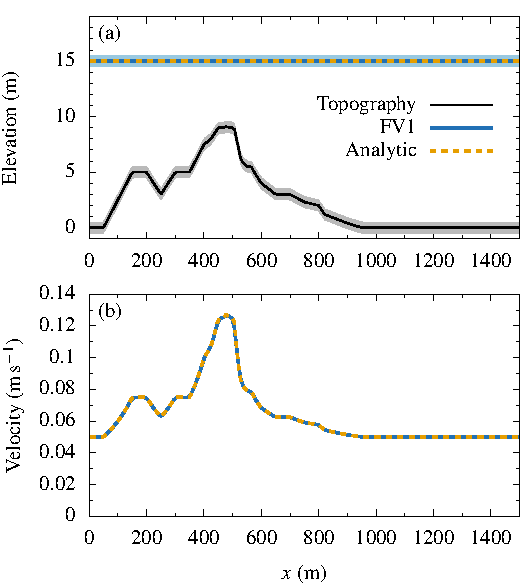
\includegraphics{fig-tsengSteadyState-flow.pdf}
    \end{subfigure}
    \caption{\rev{Steady state solution over an irregular and uncertain bed.
    (a) Bed elevation and free-surface elevation.
    Mean values are marked with solid lines, with shading indicating plus or minus one standard deviation of uncertainty.
    (b) Spatial profile of depth-average velocity.
    The mean velocity is marked with a solid line and the standard deviation of velocity is negligible.
    In both panels, the analytic mean solution is marked with a dashed yellow line.}}
    \label{fig:tsengSteadyState-flow}
\end{figure}

\rev{The stochastic Galerkin model is configured with a basis order $P=3$, and the resulting steady-state solution is shown in figure~\ref{fig:tsengSteadyState-flow}.
Since the flow is very slow, the free-surface elevation is uniform.
The free-surface elevation has the same standard deviation as the topography, which is due to the water depth at the downstream boundary being fixed at \SI{15}{\meter} with no uncertainty.
As a result, the water depth profile is certain, and the uncertainty in the free-surface elevation is determined entirely by the topography.}
\rev{The corresponding depth-averaged velocity profile is shown in figure~\ref{fig:tsengSteadyState-flow:u}.
The stochastic Galerkin model calculates a velocity profile that is in excellent agreement with the analytic solution.
The predicted velocity profile is certain with negligible standard deviation.
This is expected since the water depth profile is unaffected by the prescribed topographic uncertainty.
These results verify the robustness of the stochastic Galerkin model for flow over a highly-irregular, uncertain bed.}